%=============================================================================
%
%	Optimization in Banach Spaces
%
%	Continuos evaluation work - Block 0
%
%=============================================================================



%=============================================================================
%	Packages
%=============================================================================

\documentclass[11pt, a4paper]{article}		% document format
\usepackage{graphicx}						% package to insert graphics
\usepackage[english]{babel}
\usepackage[utf8]{inputenc}					% this enables all unicode characters
\usepackage{amsmath, amsfonts, amssymb} 	% maths packages
\usepackage{amsthm}							% theorem styles
\usepackage{fancyhdr}						% package for headers, foot and margin notes
\usepackage{enumitem}						% allows to change the enumeration format in line



%=============================================================================
%	Commands
%=============================================================================

\providecommand{\U}[1]{\protect\rule{.1in}{.1in}}
\newcommand{\N}{\mathbb{N}}
\newcommand{\E}{\mathcal{E}}
\newcommand{\R}{\mathbb{R}}



%=============================================================================
%	Environment
%=============================================================================

\theoremstyle{plain}
\newtheorem{exercise}{Exercise}
\newtheorem{algorithm*}{Algorithm}

\theoremstyle{definition}
\newtheorem{solution}{Solution}[exercise]
\renewcommand*{\thesolution}{\theexercise.\alph{solution}}	% Make solution instances enumerate with number of exercise and letter of solution




%============================================================================
%	Pagestyle
%=============================================================================

\pagestyle{fancy}		% As we use the fancyhdr pkg need the fancy pagestyle, for more information:
						% http://tug.ctan.org/tex-archive/macros/latex/contrib/fancyhdr/fancyhdr.pdf


%\topmargin 0 pt
%\oddsidemargin 0 pt
%\evensidemargin 0 pt
%\marginparwidth 0 pt


%\textheight 25cm
%\textwidth 400 pt
%\advance\textheight by \topskip

%\parindent 0pt
%\parskip 5mm plus 1mm minus 1mm

%\fancyhead[C]{Report I}					                % Central header
\fancyhead[L]{Optimization in Banach Spaces}   				% Left header
\fancyhead[R]{Marc Jovani Bertran}						    % Right header



%=============================================================================
%	Document
%=============================================================================

\begin{document}
	\section*{1}

\begin{enumerate}[label=\Alph*]
    
\item Resuelva gráficamente el siguiente problema de optimización:
        \begin{equation*}
        \begin{aligned}
            \text{Minimizar }   & x_1^2 + x_2^2 \\
            \text{sujeto a }    & x_1 \geq 0,\; x_2 \geq 0, \\
                                & x_1 x_2 \geq 1 \\
                                & x_1 + x_2 \geq 4 \\
        \end{aligned}
        \end{equation*}

\item Resuelva, ahora, el problema de maximización con la misma función objetivo y el mismo conjunto factible del apartado anterior. 

\end{enumerate}

\noindent\rule{10cm}{0.4pt}

Usando \textit{Python} junto a \textit{matplotlib} creamos un gráfico con curvas de nivel sobre el conjunto factible,
para ello damos un valor de $+\infty$ a los puntos que no cumplan con las restricciones.

Como vemos en la figura \ref{ex0_min} el mínimo se encuentra en el punto $(2, 2)$.

\begin{figure}[h]
\centering
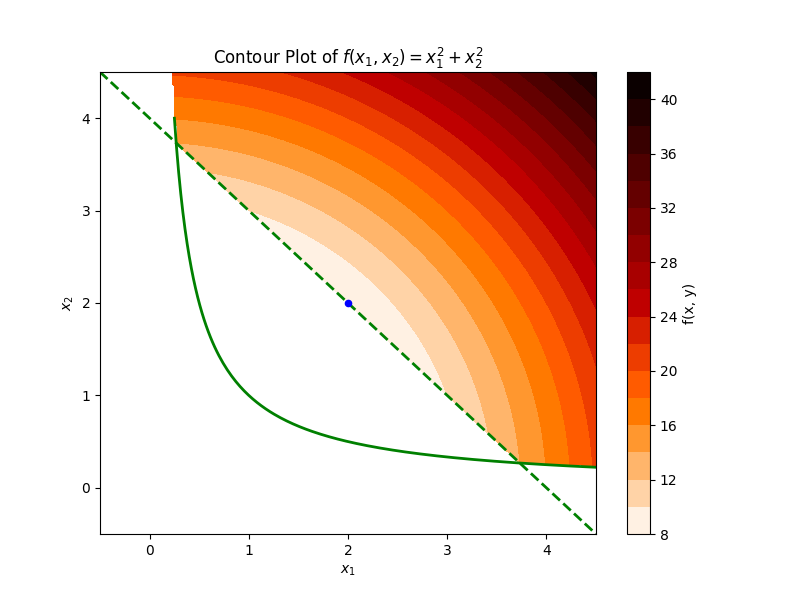
\includegraphics[scale=0.6]{ex0_min.png}
\caption{Solución gráfica para el problema de minimizar.}
\label{ex0_min}
\end{figure}

Para resolver el problema de maximización damos un valor de $-\infty$ a los puntos que no cumplan las restricciones.
Como se ve en la figura \ref{ex0_max} el funcional no esta acotado en el conjunto factible,
por tanto no tiene solución.

\begin{figure}[h]
\centering
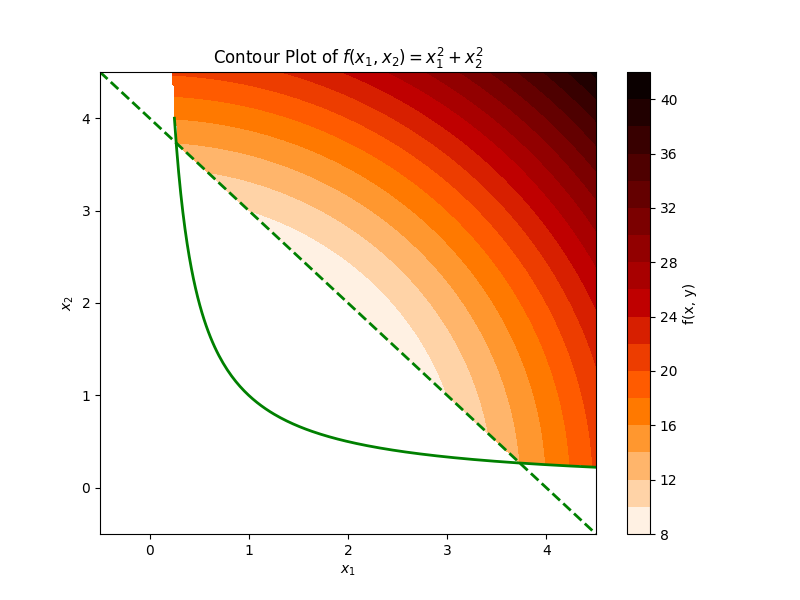
\includegraphics[scale=0.6]{ex0_max.png}
\caption{Solución gráfica para el problema de maximización.}
\label{ex0_max}
\end{figure}


	\section*{2}

Dado el conjunto $M \subset \R^2$ definido por
\begin{equation*}
    M = \{(x_1 , x_2 ) \in \R^2 : x_1 \leq x_2 , x_2 \leq -x_1^2 + 2\},
\end{equation*}
se considera la función de $\R^2$ en $\R$ que a cada punto de $\R^2$ le asocia su distancia al origen,
y se trata de obtener los puntos de M cuya distancia al origen es máxima y mínima.
Formule el problema de optimización, indicando la función objetivo y el conjunto factible y resuélvalo gráficamente utilizando curvas de nivel.

\noindent\rule{10cm}{0.4pt}

Para obtener los puntos de $M$ cuya distancia al origen es minima planteamos el siguiente problema de optimización,
\begin{equation} \label{ex1_min_implicit}
\begin{aligned}
    \text{Minimizar }   & x_1^2 + x_2^2 \\
    \text{sujeto a }    & (x_1, x_2) \in M,
\end{aligned}
\end{equation}
donde la funcion objetivo es $x_1^2 + x_2^2$ y el conjunto factible es $M$.

Podemos hacer que las restricciones del problema \ref{ex1_min_implicit} sean explicitas,
\begin{equation} \label{ex1_min_explicit}
\begin{aligned}
    \text{Minimizar }   & x_1^2 + x_2^2 \\
    \text{sujeto a }    & x_1 \leq x_2, \\
                        & x_2 \leq -x_1^2 + 2.
\end{aligned}
\end{equation}

Resolviendo el problema \ref{ex1_min_explicit} gráficamente usando \textit{Python} y \textit{matplotlib}
vemos que el problema tiene un único mínimo localizado en el origen, como vemos en al figura \ref{ex1_min}.

\begin{figure}[h]
\centering
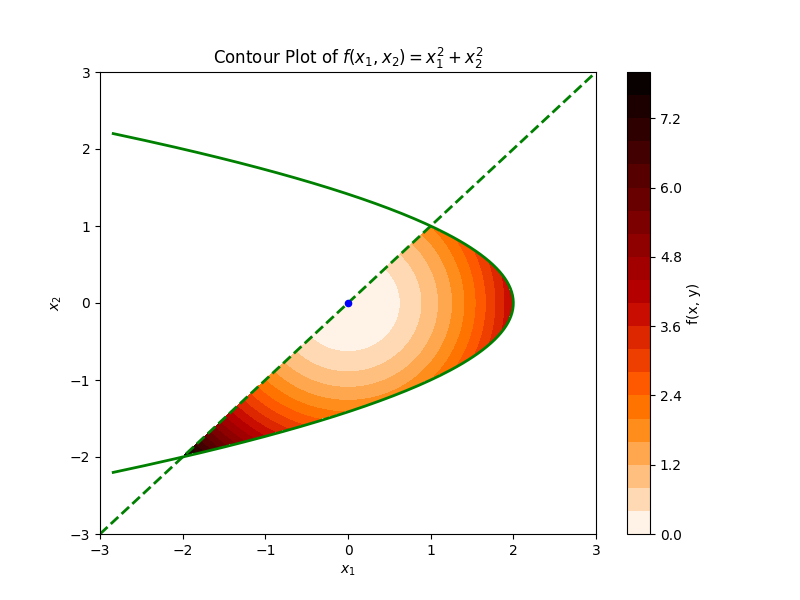
\includegraphics[scale=0.6]{ex1_min.png}
\caption{Solución gráfica para el problema de minimizar.}
\label{ex1_min}
\end{figure}

Para encontrar el punto con distancia maxima al origen planteamos el siguiente problema de maximización.
\begin{equation} \label{ex1_max_explicit}
\begin{aligned}
    \text{Maximizar }   & x_1^2 + x_2^2 \\
    \text{sujeto a }    & x_1 \leq x_2, \\
                        & x_2 \leq -x_1^2 + 2.
\end{aligned}
\end{equation}

Resolviendo el problema \ref{ex1_max_explicit} gráficamente,
obteniendo la figura \ref{ex1_max} 
y vemos que el problema tiene un único mínimo localizado en el el punto $(-2,-2)$.

\begin{figure}[h]
\centering
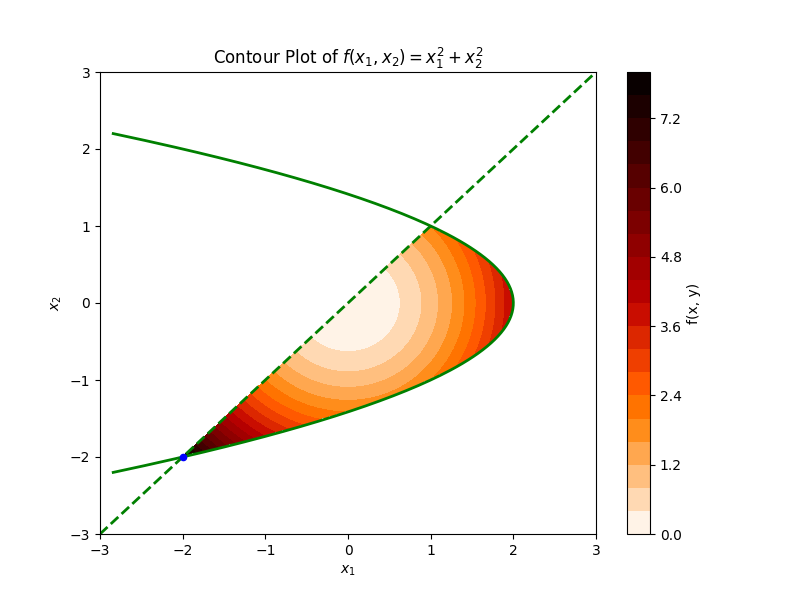
\includegraphics[scale=0.6]{ex1_max.png}
\caption{Solución gráfica para el problema de minimizar.}
\label{ex1_max}
\end{figure}

	\section*{3}

Una persona dispone de 6000 euros para invertir.
Se le sugiere invertir en bonos de dos tipos A y B.
Los del tipo A tienen más riesgo y dan un interés anual del 10\%,
mientras que los del tipo B tienen menos riesgo, pero dan un interés anual del 7\%.
Esta persona decide invertir, como máximo, 3500 euros en bonos del tipo A,
y 2400 euros, como mínimo, en bonos del tipo B,
de forma que la cantidad invertida en bonos de tipo A no sea menor que la invertida en bonos de tipo B.
Su objetivo es obtener, con estas restricciones, el máximo interés.

Se pide formular el correspondiente problema de optimización.

\noindent\rule{10cm}{0.4pt}

Sean $e_A$ la cantidad de euros invertidos en bonos del tipo $A$ y $e_B$ la cantidad de euros invertidos en bonos del tipo $B$,
la función objetivo representa el interés anual que se va a recibir,
esta esta representada por $\frac{0.1 e_A + 0.07 e_B}{e_A + e_B}$,
suponiendo que ninguno de los dos bonos deja de pagar.

Por otro lado las restricciones que tenemos que tener en cuenta son no sobre pasar el capital total,
respetar el máximo y mínimo a invertir en los bonos del tipo $A$ y $B$,
y que la inversion en bonos del tipo $A$ no sea menor a la del tipo $B$.

Con todo esto tenemos el problema de optimización,
\begin{equation}
\begin{aligned}
    \text{Maximizar }   & \frac{0.1 e_A + 0.07 e_B}{e_A + e_B} \\
    \text{sujeto a }    & e_A + e_B \leq 6000 \\
                        & e_A \leq 3500 \\
                        & e_B \geq 2400 \\
                        & e_A \geq e_B \\
\end{aligned}
\end{equation}

\end{document}